\documentclass[12pt]{article} % use larger type; default would be 10pt
\usepackage[utf8]{inputenc} % set input encoding (not needed with XeLaTeX)

%%% PAGE DIMENSIONS
\usepackage{geometry} % to change the page dimensions
\geometry{a4paper} % or letterpaper (US) or a5paper or....
\geometry{margin=2cm} % or letterpaper (US) or a5paper or....

\usepackage{graphicx} % support the \includegraphics command and options
\usepackage[parfill]{parskip} % Activate to begin paragraphs with an empty line rather than an indent
\usepackage{times} % for Times Roman default font

%%% PACKAGES
\usepackage{booktabs} % for much better looking tables
\usepackage{array} % for better arrays (eg matrices) in maths
\usepackage{paralist} % very flexible & customisable lists (eg. enumerate/itemize, etc.)
\usepackage{verbatim} % adds environment for commenting out blocks of text & for better verbatim
\usepackage{subfig} % make it possible to include more than one captioned figure/table in a single float

%%% HEADERS & FOOTERS
\usepackage{fancyhdr} % This should be set AFTER setting up the page geometry
\pagestyle{fancy} % options: empty , plain , fancy
\renewcommand{\headrulewidth}{0pt} % customise the layout...
\lhead{}\chead{}\rhead{}
\lfoot{}\cfoot{\thepage}\rfoot{}

\makeatletter
\renewcommand{\maketitle}{%
  {\bfseries{\scshape{\Large{\@title\par}}}}
}
\makeatother

\hyphenation{Kiwi-bank} % otherwise it may get hyphenated as Ki-wibank

%%% END Article customizations

%%% The "real" document content comes below...

\title{Travers Peak: 6 May 2017 \footnotesize{(Alisa's 37th birthday)}}

\begin{document}
  \maketitle

Left the carpark at 10:20.  Lovely and clear on the East side of the Pass, although the bach (house) was under a layer of high fog which appeaed to have only just dispersed when we got back (about 16:00).  We had lunch just above the bushline, after which we decided to go on `towards the top'.  Not surprisingly, we went all the way.  There was still a bit of snow from the fall a couple of nights earlier.

On the way back down, I startled a chamois coming up the path - about 10 minutes up from `Moa Point'.  A great day - back to the car at 15:20 (i.e., 5 hours, including lunch).

\begin{flushright}
Lilly, Kevin, Robyn, Peter and dog
\end{flushright}

\begin{figure}[ht]
%\centering
\begin{minipage}{.5\linewidth}
\begin{flushleft}
   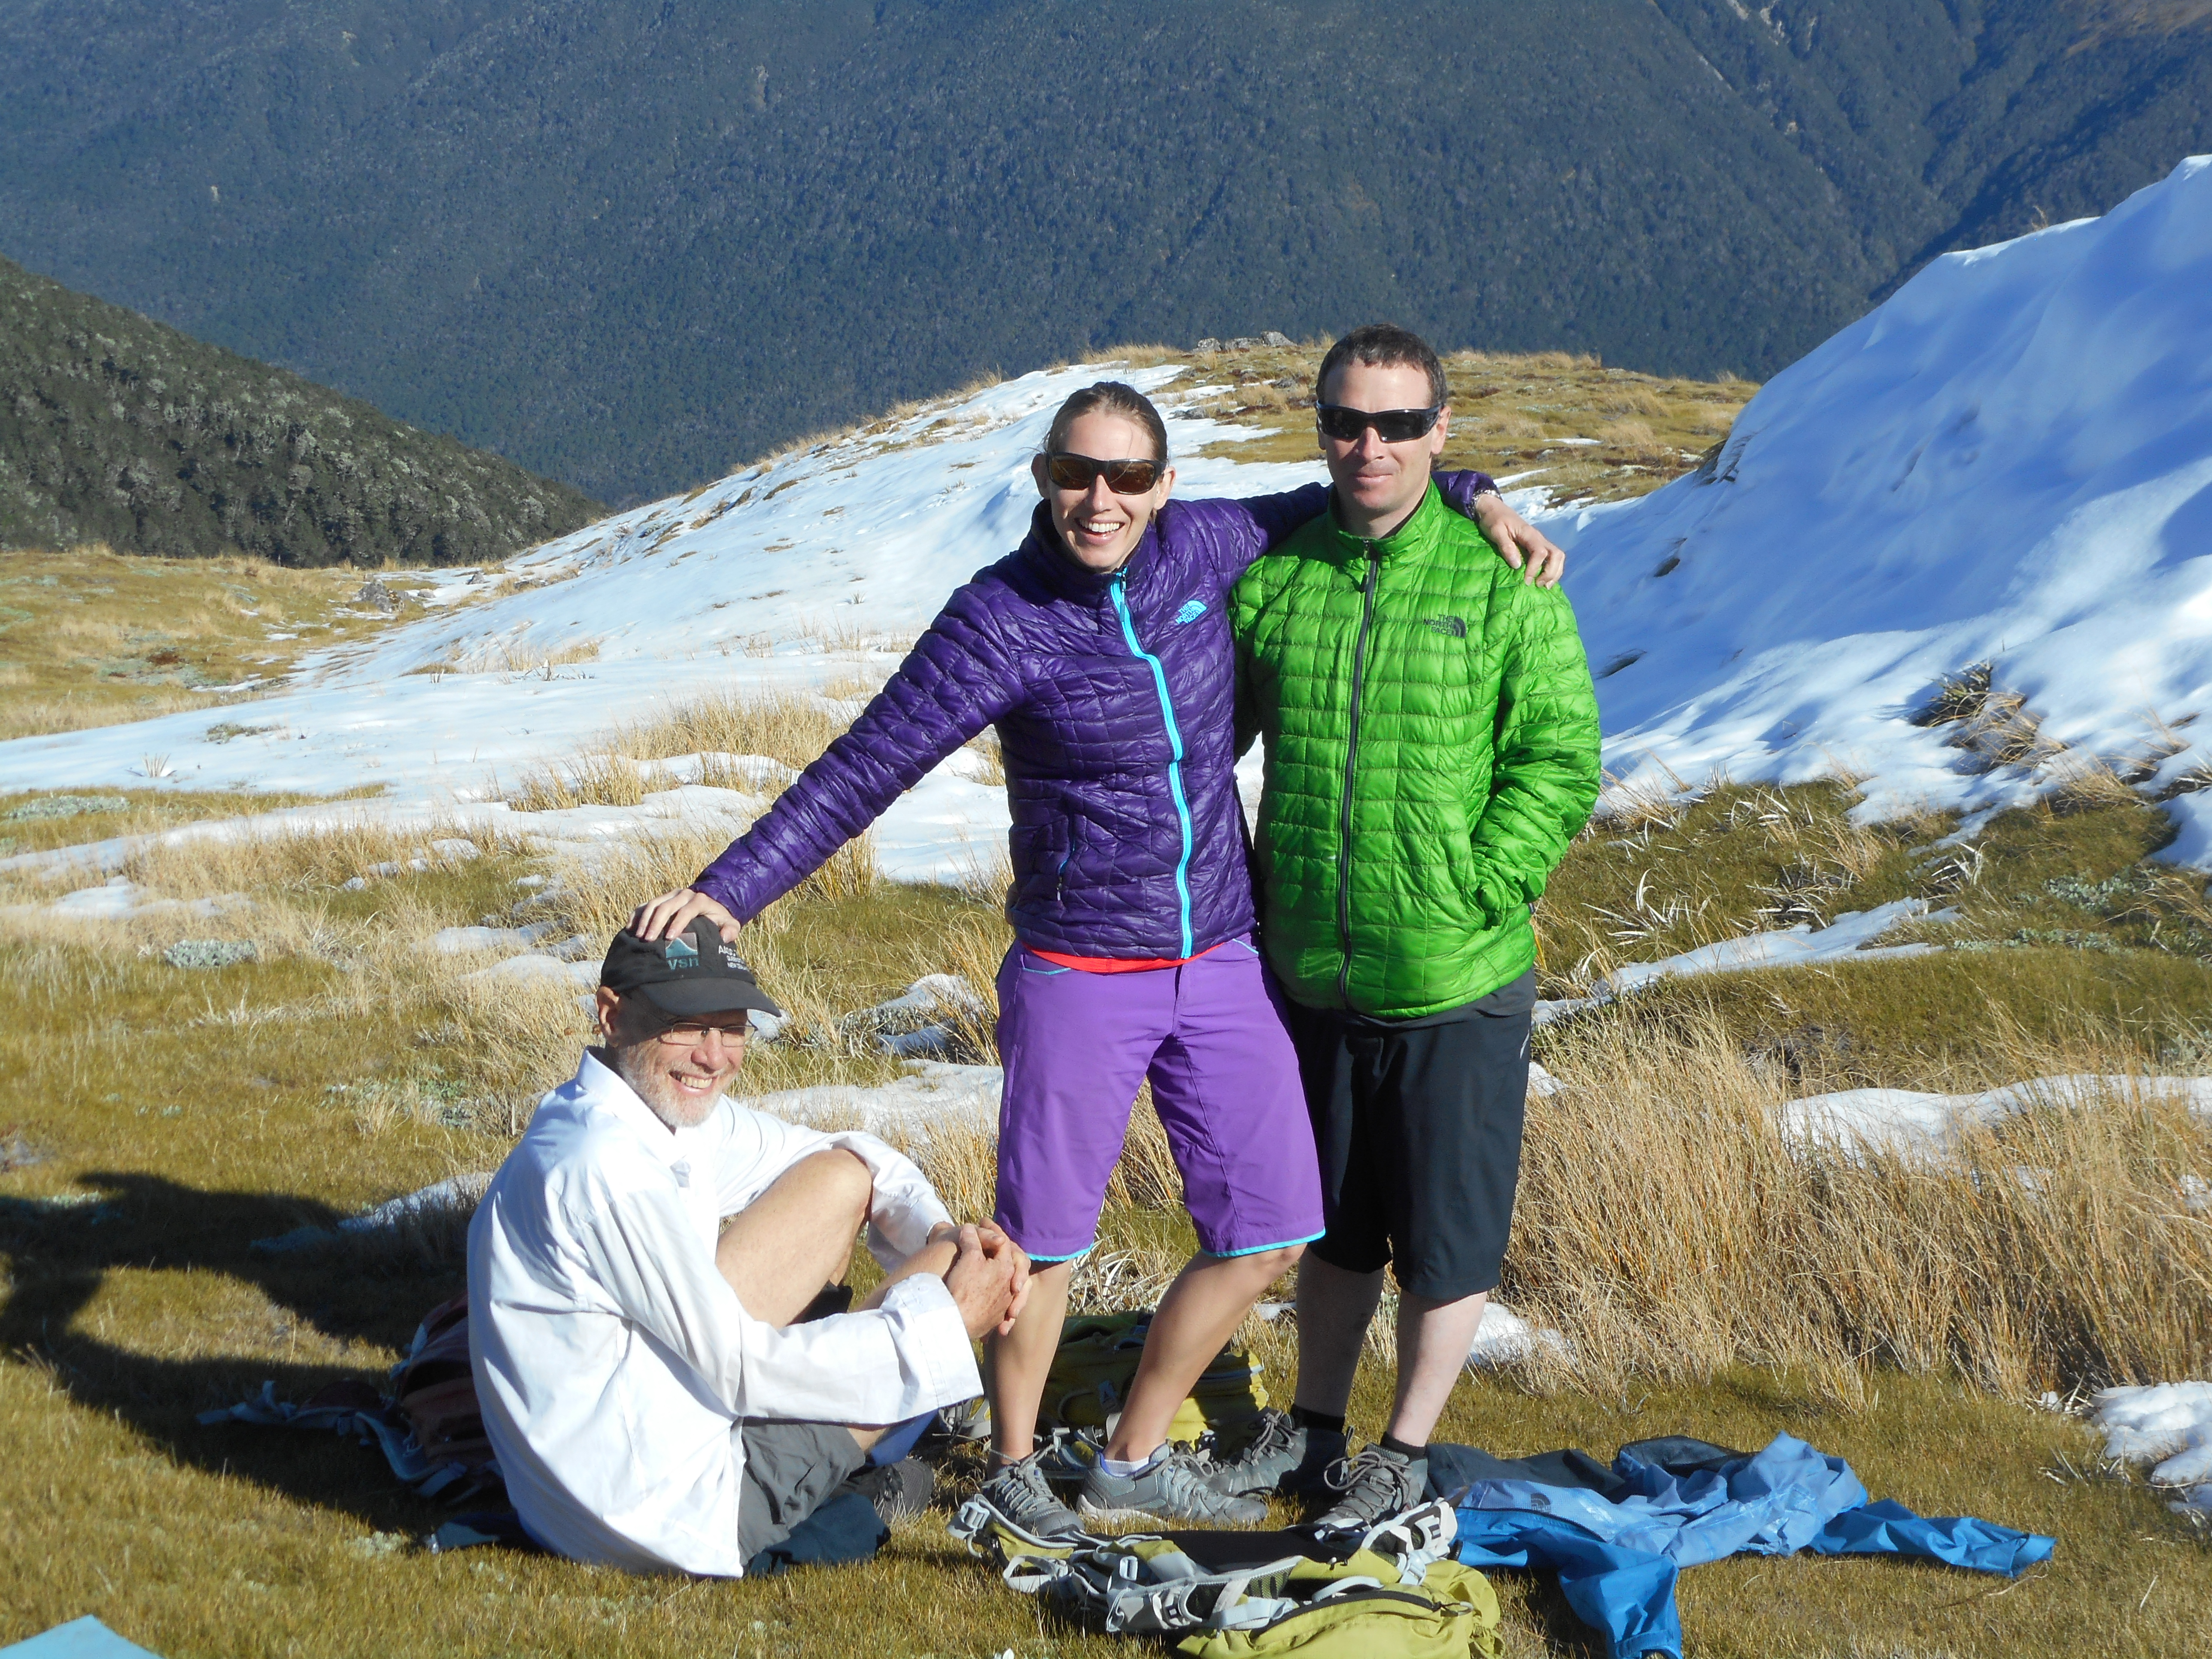
\includegraphics[width=8cm]{TraversPeak06May2017Photo1}
\end{flushleft}
\end{minipage}
\begin{minipage}{.5\linewidth}
\begin{flushright}
    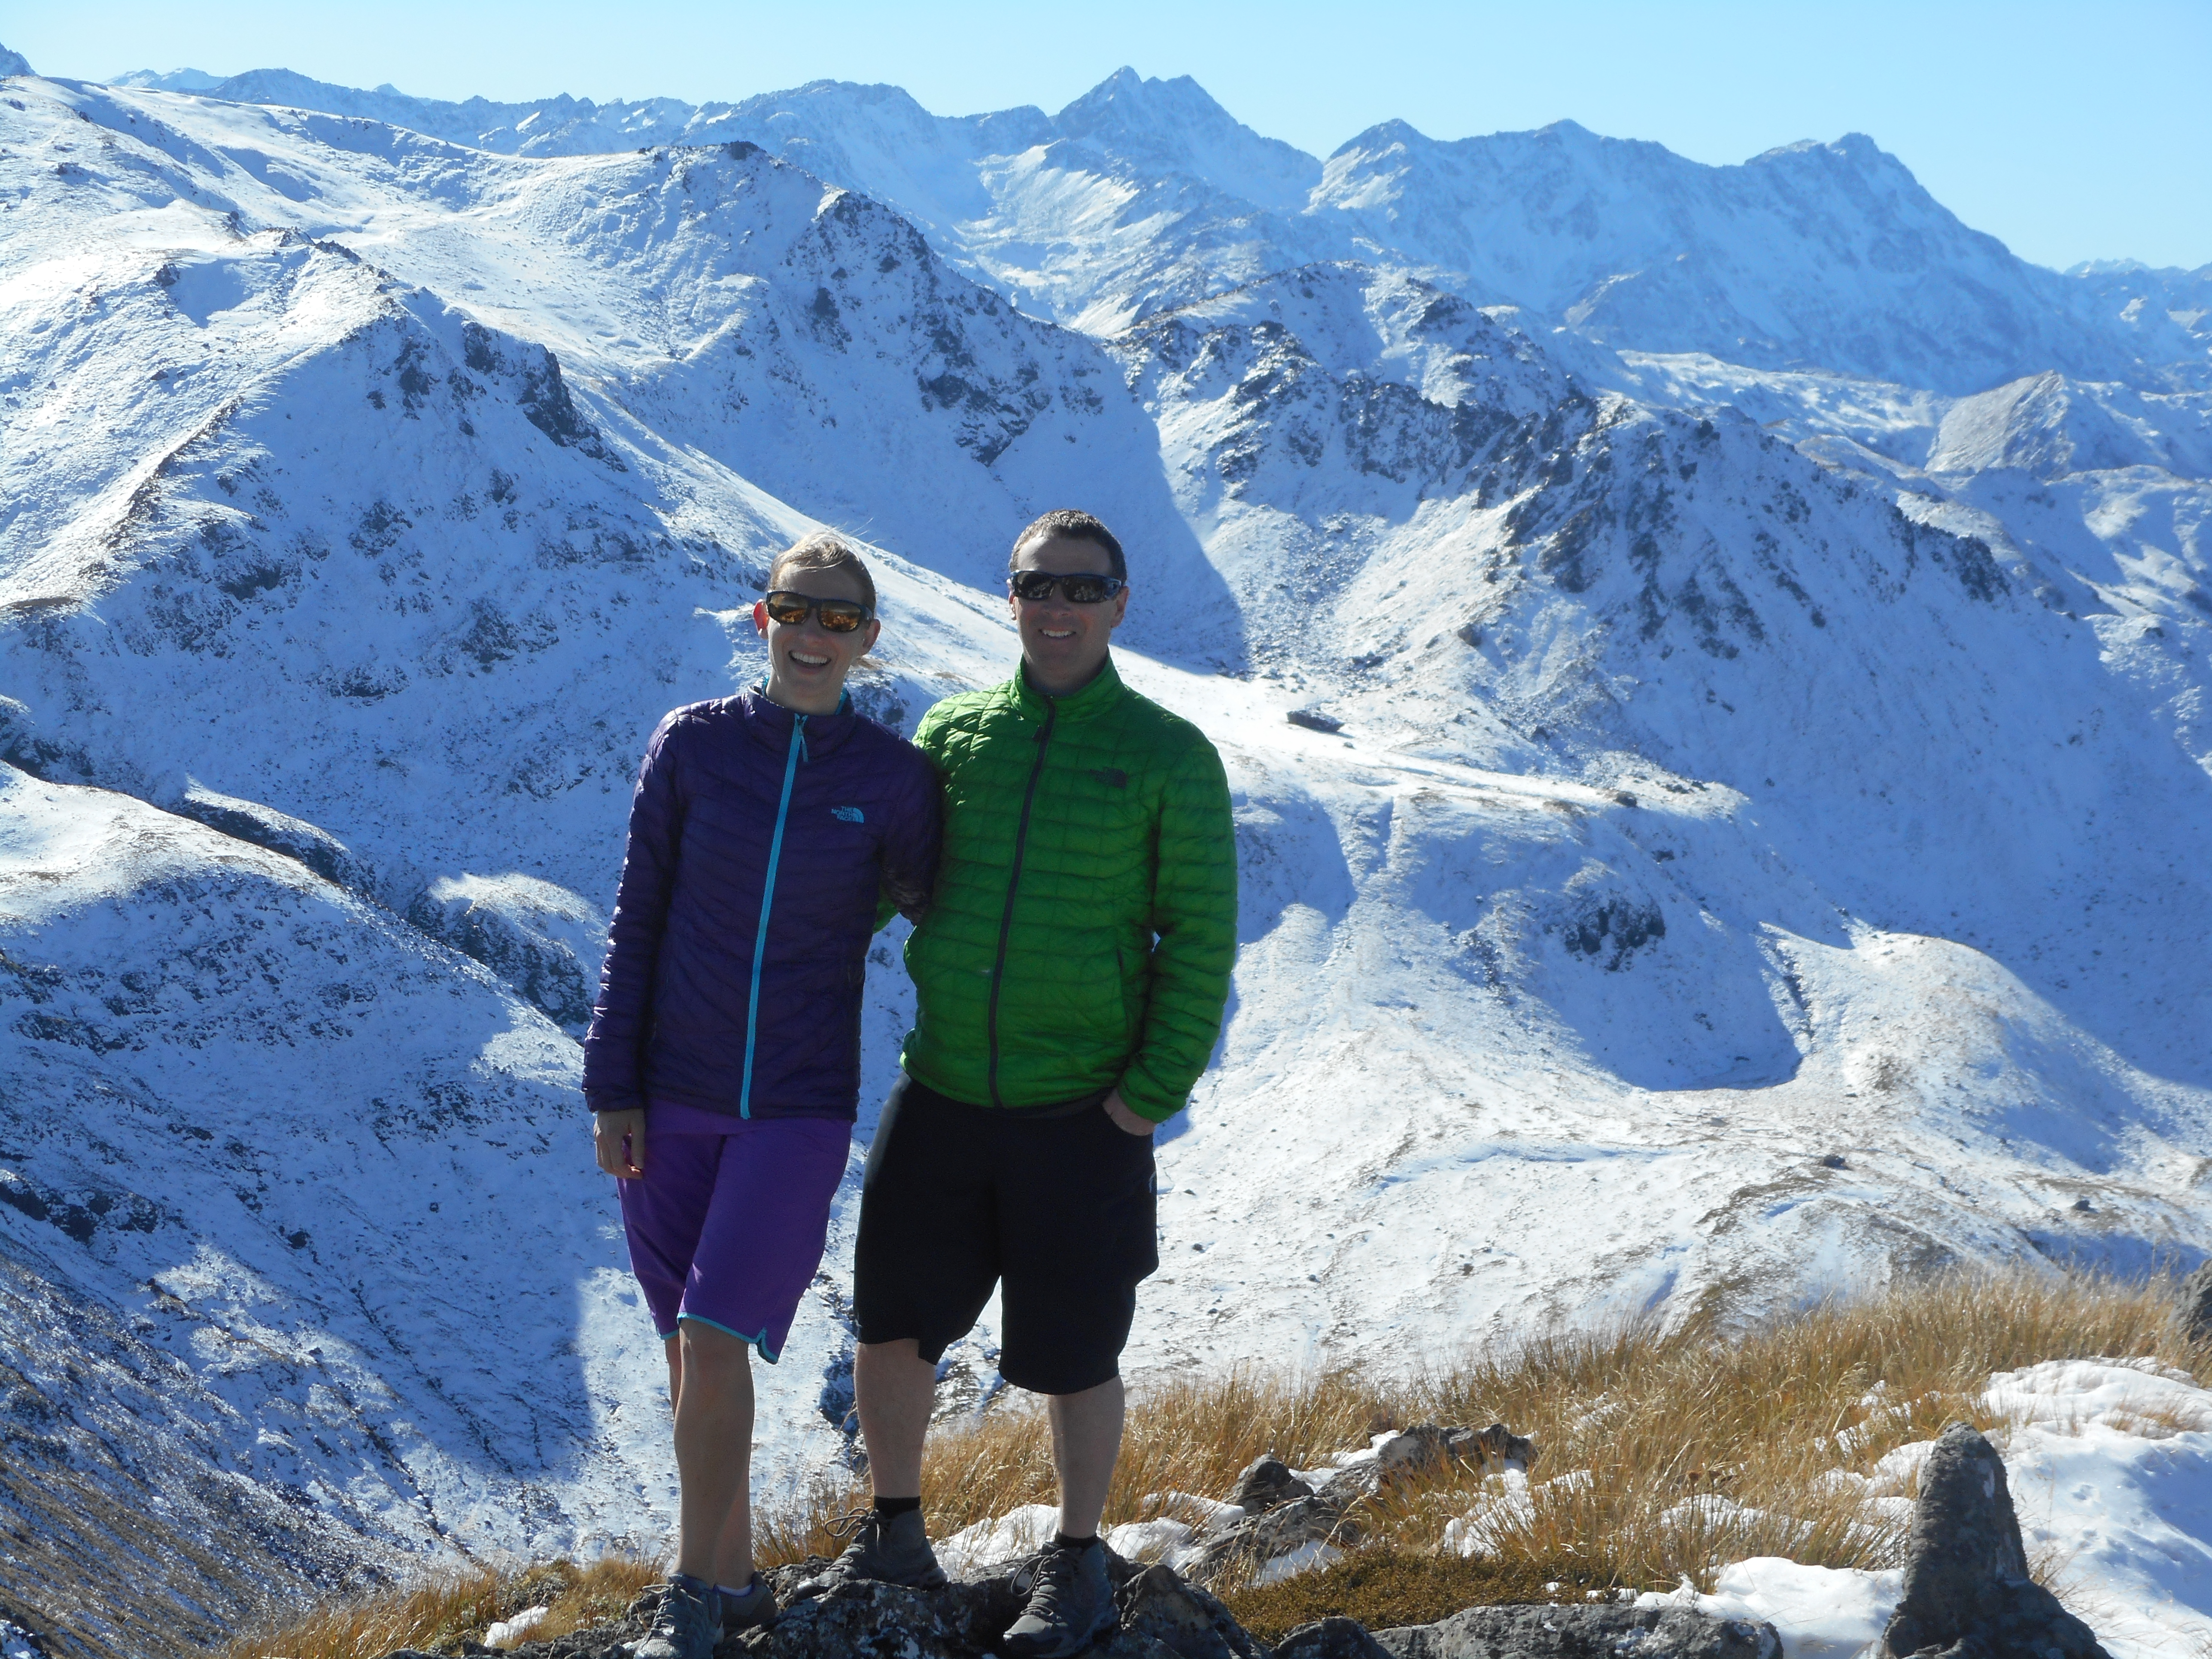
\includegraphics[width=8cm]{TraversPeak06May2017Photo2}
\end{flushright}
\end{minipage}
\end{figure}

\end{document}
